\begin{frame}{Formule de Künneth}
Pour toutes $C^*$-algèbres $A$ et $B$, on définit
\[\alpha_{A,B} : K_*(A)\otimes K_*(B)\rightarrow K_*(A\otimes B) \quad ; \quad (x,y)\mapsto x\otimes   \tau_A(y).\]

\begin{definitionfr}
Une $C^*$-algèbre $A$ satisfait la formule de Künneth si, pour toute $C^*$-algèbre $B$ telle que $K_*(B)$ soit libre, $\alpha_{A,B}$ est un isomorphisme.
\end{definitionfr}

Si $A$ satisfait la formule de Künneth, alors, pour toute $C^*$-algèbre $B$, la suite suivante
\[0  \rightarrow K_*(A)\otimes K_*(B) \rightarrow K_*(A\otimes B)  \rightarrow Tor(K_*(A),K_*(B)) \rightarrow 0\]
est exacte.

\end{frame}

\begin{frame}{Formule de Künneth}
Si $A$ est $\mathcal E$-filtrée, $A\otimes B$ est $\mathcal E$-filtrée par $\{A_E\otimes B\}_E$. Pour tout $z \in KK(B_1,B_2)$, on dispose d'un morphisme contrôlé 
\[\hat \tau_A (z): K^{\varepsilon,E}(A\otimes B_1 ) \rightarrow K^{\alpha_\tau\varepsilon,k_\tau(\varepsilon).E}(A\otimes B_2)\]
qui induit $-\otimes \tau_A(z) $ en $K$-théorie \cite{OY2}.\\
\vspace{0.3 cm}
On définit le morphisme contrôlé  
\[\hat\alpha_{A,B} : \hat K_*(A)\otimes K_*(B)\rightarrow \hat K_*(A\otimes B) \quad ; \quad (x,y)\mapsto \hat\tau_A(y)(x),\]
qui induit donc $\alpha_{A,B}$ en $K$-théorie.\\
\end{frame}

\begin{frame}{Formule de Künneth}
Le morphisme contrôlé $\hat\alpha_{A,B}$ est dit :
\vspace{0.3 cm}
\begin{itemize}
 
\item[$\bullet$] quasi-injectif s'il existe $\lambda \geq 1$ tel que, pour tout $\varepsilon\in (0,\frac{1}{4\alpha_\tau \lambda})$ et $F\in\mathcal E$, il existe $F'\in\mathcal E$, et $F\subseteq F'$, tels que: 
\[\forall x\in K^{\varepsilon,F}(A)\otimes K(B)\text{ t.q. }\alpha_{A,B}^{\varepsilon,F}(x)=0 \text{ alors }(\iota_{\varepsilon,F}^{\lambda\varepsilon,F'}\otimes id) (x) = 0.\] 

\item[$\bullet$] quasi-surjectif s'il existe $\lambda \geq 1$ tel que, pour tout $\varepsilon \in (0,\frac{1}{4\alpha_\tau})$ et $F\in\mathcal E$, il existe $F'\in\mathcal E$, $F\subseteq h_{\tau,\lambda\varepsilon}.F'$, tels que:
\[ \forall y\in K^{\varepsilon,F}(A\otimes B), \exists x\in K^{\lambda\varepsilon, F'}(A)\otimes K(B) \text{ t.q. }\]
\[\alpha^{\lambda\varepsilon,F'}_{A,B}(x)=\iota_{\varepsilon,F}^{\alpha\lambda\varepsilon,h_{\tau, \lambda\varepsilon}.F'}(y).\] 

\end{itemize}
\end{frame}

\begin{frame}{Formule de Künneth}
\begin{definitionfr}
Une $C^*$-algèbre $\mathcal E$-filtrée $A$ satisfait la formule de Künneth quantitative s'il existe $\lambda \geq 1$ tel que, pour toute $C^*$-algèbre $B$ telle que $K_*(B)$ soit libre, $\hat\alpha_{A,B}$ est quasi-injectif et quasi-surjectif. 
\end{definitionfr}

Si $A$ satisfait la formule de Künneth quantitative, alors elle satisfait la formule de Künneth usuelle.\\
\vspace{0.3 cm}
\textbf{Remarque :} l'intêret de la formule de Künneth quantitative est qu'elle est stable par des décompositions plus faibles que la formule usuelle. (Oyono-Oyono \& Yu, 2016 \cite{OY4}).
\end{frame}

\begin{frame}{Formule de Künneth}
\[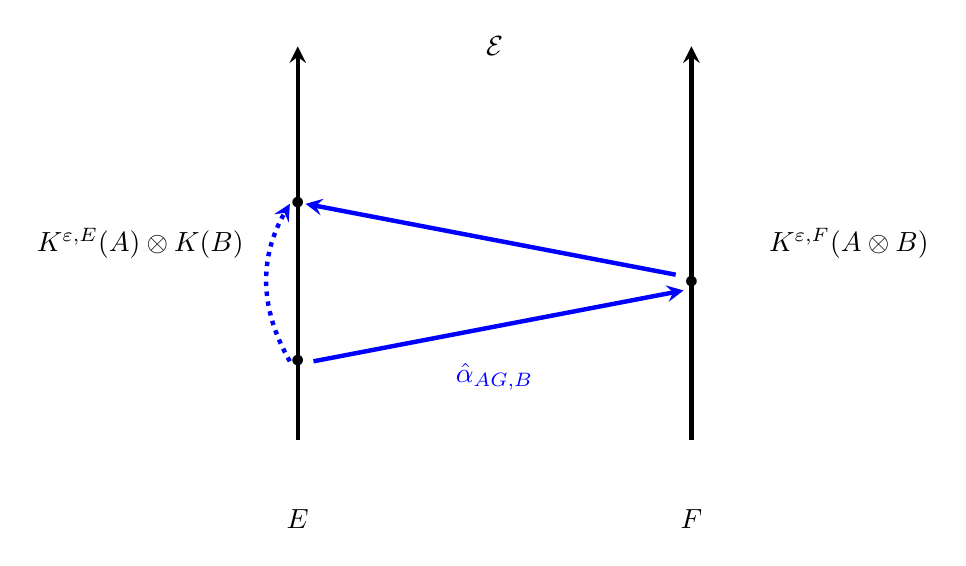
\begin{tikzpicture}
\draw  (2.5,5) node {$\mathcal E$};
\draw  (0,-1) node {$E$};
\draw  (5,-1) node {$F$};
\draw  (-2,2.5) node {$K^{\varepsilon,E}(A)\otimes K(B)$};
\draw  (7,2.5) node {$K^{\varepsilon,F}(A\otimes B)$};
\draw [>=stealth, ->,ultra thick] (0,0) -- (0,5) ; %->
\draw [>=stealth, ->,ultra thick] (5,0) -- (5,5) ; 

\pause
\draw  (0,1) node {$\bullet$};
\draw  (5,2) node {$\bullet$};
\draw [>=stealth, ->,ultra thick, blue] (0.2,1) -- (4.9,1.9) ; 
\draw[blue] (2.5,0.8) node {$\hat\alpha_{A\rtimes G,B}$};

\pause
\draw  (0,3) node {$\bullet$};
\draw [>=stealth, ->,ultra thick, blue] (4.8,2.1) -- (0.1,3) ; 

\pause
\draw [>=stealth, ->,ultra thick, blue, dotted] (-0.1,1) to[bend left] (-0.1,3) ; 

\end{tikzpicture}\]
\end{frame}

\begin{frame}{Formule de Künneth}
On veut démontrer que, sous de bonnes conditions,  
\[\alpha_{A\rtimes_r G,B} : K(A\rtimes_r G)\otimes K(B) \rightarrow K((A\rtimes_r G)\otimes B)\]
est un isomorphisme pour toute $C^*$-algèbre $B$ telle que $K(B)$ soit libre.\\
\vspace{0.3 cm}
\textbf{Stratégie:}
\begin{itemize}
\item[$\bullet$] définir une version topologique 
\[\alpha_{A,B}^{G} : K^{top}(G,A)\otimes K(B) \rightarrow K^{top}(G,A\otimes B)\]
de $\alpha_{A\rtimes_r G,B}$.
\item[$\bullet$] montrer que l'application d'assemblage les entrelace.
\item[$\bullet$] se ramener au cas de certains sous-groupoïdes de $G$ par restriction.
\end{itemize}
\end{frame}

\begin{frame}{Formule de Künneth}
La classe $\mathcal C$ définit une classe de groupoïdes dont toutes les actions propres sont localement induites par des sous-groupoïdes compacts ouverts. 
\vspace{0.3 cm}
\begin{definitionfr}
Un groupoïde étale $G$ est dans la classe $\mathcal C$ si, pour toute action propre $G$ sur un espace $Z$, il existe un recouvrement ouvert $\mathcal U$ de $Z$ tel que, pour tout $U\in\mathcal U$, il existe un sous-groupoïde compact ouvert $H_U$ de $G$ et un $H_U$-espace $Z_U$ et un homéomorphisme $G$-equivariant
\[\psi_U : U \rightarrow G\times_{H_U} Z_U.\] 
\end{definitionfr}
\vspace{0.3 cm}
\textbf{Exemples:} les groupes discrets, les groupoïdes amples (J. Renault).

\end{frame}


\begin{frame}{Formule de Künneth}
\begin{thmfr}
Soit $G$ un groupoïde $\sigma$-compact étale et $A$ une $G$-algèbre. Si 
\begin{itemize}
\item[$\bullet$] $G$ vérifie la conjecture de Baum-Connes à coefficients,
\item[$\bullet$] $G$ est dans la classe $\mathcal C$,
\item[$\bullet$] pour tout sous-groupoïde compact ouvert $H$ de $G$ et tout $H$-espace $V$ telle que l'application moment $p : V\rightarrow H^{(0)}$ soit localement injective, $\alpha_{A,B}^{H,V}$ est un isomorphisme.
\end{itemize} 
Alors $A\rtimes_r G$ vérifie la formule de Künneth contrôlée.
\end{thmfr}
\end{frame}

\begin{frame}{Idée de la preuve}
On définit  
\[\alpha_{A,B}^{G,Z} : RK^G(Z,A)\otimes K(B) \rightarrow RK^G(Z,A\otimes B)\]
pour toute $G$-algèbre $A$, $C^*$-algèbre $B$ et $G$-espace $Z$.
Le diagramme suivant commute :
\[\begin{tikzcd}[ampersand replacement=\&, column sep=small] 
\alpha_{A,B}^{G,P_E}: RK^G(P_E,A)\otimes K(B)\arrow{r}\arrow{d}{\mu_{G,A}\otimes id}    \& RK^G(P_E,A\otimes B)\arrow{d}{\mu_{G,A\otimes B}} \\
\alpha_{A\rtimes_r G,B}: K(A\rtimes_r G) \otimes K(B) \arrow{r} \& K((A\rtimes_r G)\otimes B)
\end{tikzcd}\]
\end{frame}

\begin{frame}{Idée de la preuve}
\begin{thmfr}
Soit $G$ un groupoïde de la classe $\mathcal C$, et soit $E\in\mathcal E$. Si, pour tout 
\begin{itemize}
\item[$\bullet$] sous-groupoïde compact ouvert $H$ de $G$
\item[$\bullet$] tout $H$-espace $V$ tel que l'application moment $p : V\rightarrow H^{(0)}$ soit localement injective,
\end{itemize} 
$\alpha_{Res_H^G(A),B}^{H,V}$ est un isomorphisme, alors 
\[\alpha_{A,B}^{G,P_E}: RK^G(P_E,A)\otimes K(B)\rightarrow RK^G(P_E,A\otimes B) \] 
est un isomorphisme pour toute $C^*$-algèbre $B$ telle que $K_*(B)$ est un groupe abélien libre.\\
\end{thmfr}
\end{frame}

\begin{frame}{Idée de la preuve}
$P_E$ possède une structure de $G$-complexe simplicial fini. (J-L. Tu).\\
\vspace{0.3 cm}
Soit $Z_0 \subseteq ...\subseteq Z_n$ la décomposition en squelette de $P_E$. Par un argument de type Mayer-Vietoris, il suffit de le démontrer pour $Z_0 = G$. Mais $p =r : Z_0 \rightarrow G^{(0)} $ est localement injective. \\
\vspace{0.3 cm}
\begin{lemfr}
Soit $H$ un sous-groupoïde compact ouvert de $G$, et $V$ un $H$-espace tel que l'application moment 
\[p: V\rightarrow H^{(0)}\] 
soit localement injective. Alors, pour tout $G$-algèbre $B$, on a un isomorphisme de groupes abéliens $\Z_2$-gradués
\[RK^G(G\times_H V,B)\cong RK^H(V,B).\]
\end{lemfr}
\end{frame}

\begin{frame}{Idée de la preuve}
Le lemme précédent se montre en définissant l'induction sur les groupoïdes étales.\\
\vspace{0.3 cm}
On peut ensuite refaire la preuve avec l'application d'assemblage contrôlée
\[\mu_{G,A}^{\varepsilon, E,E'} : RK^G(P_E,A)\rightarrow K^{\varepsilon,E'}(A\rtimes_r G)\]
pour obtenir la version contrôlée du résultat.
\end{frame}

